\documentclass[12pt,a4paper]{article}
\usepackage[utf8]{inputenc}
\usepackage[T1]{fontenc}
\usepackage[italian]{babel}
\usepackage{geometry}
\usepackage{amsmath}
\usepackage{amssymb}
\usepackage{listings}
\usepackage{xcolor}
\usepackage{graphicx}
\usepackage{hyperref}
\usepackage{booktabs}
\usepackage{caption}
\usepackage{float}
\usepackage{parskip}
\usepackage{array}
\usepackage{tabularx}
\usepackage{tcolorbox}
\tcbuselibrary{listings,breakable,skins}

\geometry{
  top=2.5cm, bottom=2.5cm,
  left=2.5cm, right=2.5cm
}

\definecolor{codebg}{RGB}{248,248,248}
\definecolor{keywordcolor}{RGB}{0,0,180}
\definecolor{commentcolor}{RGB}{0,128,0}
\definecolor{stringcolor}{RGB}{163,21,21}
\definecolor{codeframe}{RGB}{180,180,180}

\lstdefinestyle{python}{
  language=Python,
  basicstyle=\ttfamily\footnotesize,
  keywordstyle=\color{keywordcolor}\bfseries,
  commentstyle=\color{commentcolor}\itshape,
  stringstyle=\color{stringcolor},
  numberstyle=\tiny\color{gray},
  numbers=left,
  stepnumber=1,
  breaklines=true,
  breakatwhitespace=false,
  showstringspaces=false,
  tabsize=4,
  xleftmargin=1.5em,
  keepspaces=true,
  columns=flexible,
  frame=none,
  aboveskip=0pt,
  belowskip=0pt,
}
\lstset{style=python}

\hypersetup{
  colorlinks=true,
  linkcolor=blue!60!black,
  urlcolor=blue!60!black,
}

\newtcblisting{pylisting}[1][]{
  listing only,
  enhanced,
  colback=codebg,
  colframe=codeframe,
  coltitle=black,
  fonttitle=\small\itshape,
  attach boxed title to top left={yshift=-2mm, xshift=4mm},
  boxed title style={colback=codebg, colframe=codeframe, boxrule=0.5pt},
  boxrule=0.5pt,
  arc=2pt,
  left=4pt, right=4pt, top=8pt, bottom=4pt,
  listing options={style=python},
  before upper={\vspace{-2pt}},
  #1
}

\newcommand{\HRule}{\rule{\linewidth}{0.5mm}}

\begin{document}
\raggedbottom

% ============================================================
% FRONTESPIZIO
% ============================================================
\begin{titlepage}
  \centering
  \vspace*{1.5cm}

  {\Large\textbf{Universit\`a degli Studi di Torino}\\[0.3em]
  Corso di Laurea Magistrale in Informatica}

  \vspace{1cm}
  \HRule\\[0.4em]
  {\LARGE\textbf{Tecnologie del Linguaggio Naturale}}\\[0.3em]
  {\large Parte 3 -- Prof.\ Luigi Di Caro}\\[0.2em]
  \HRule

  \vspace{1.2cm}
  {\huge\textbf{Lab 3}}\\[0.5em]
  {\LARGE Complessit\`a Polisemica Cross-Linguistica}\\[0.4em]
  {\large Confronto della polisemia tra Inglese, Italiano e Spagnolo tramite Open Multilingual WordNet}

  \vspace{2cm}

  {\large\textbf{Gruppo di lavoro:}}\\[0.8em]
  \begin{tabular}{ll}
    \toprule
    \textbf{Studente}    & \textbf{Matricola} \\
    \midrule
    Alessandro Olivero   & 915069  \\
    Samuele Iudice       & 1235245 \\
    Andrea Franco        & 1226739 \\
    \bottomrule
  \end{tabular}

  \vspace{1.5cm}
  \begin{tabular}{ll}
    \textbf{Docente:}          & Prof.\ Luigi Di Caro \\[0.3em]
    \textbf{Anno Accademico:}  & 2025/2026 \\
  \end{tabular}

  \vfill
\end{titlepage}

\tableofcontents
\newpage

% ============================================================
\section{Introduzione}
% ============================================================

Questo laboratorio affronta il \textbf{Progetto 3: Confronto cross-linguistico} proposto nelle dispense del corso (Capitolo 4, ``Polisemia: complessit\`a, struttura e variazioni multilingue''). L'obiettivo \`e verificare empiricamente una delle tesi centrali del capitolo: \emph{la polisemia non \`e una propriet\`a universale della parola, ma del modo in cui una lingua organizza il proprio lessico}. Non esiste cio\`e una ``polisemia assoluta'' indipendente dalla lingua -- la stessa area concettuale pu\`o essere lessicalizzata in modo completamente diverso da una lingua all'altra.

Per verificarlo, si confronta la complessit\`a polisemica di \textbf{20 lemmi} (8 sostantivi, 6 verbi, 6 aggettivi) tradotti in \textbf{tre lingue} -- inglese, italiano e spagnolo -- usando l'Open Multilingual WordNet (OMW) tramite NLTK. Per ciascuna lingua si misura il numero di sensi (synset) e si calcola l'entropia di Shannon della loro distribuzione, per poi confrontare i risultati e individuare i lemmi con \textbf{asimmetria cross-linguistica} pi\`u marcata.

% ============================================================
\section{Background Teorico}
% ============================================================

\subsection{Le tre dimensioni della polisemia}

Seguendo l'impostazione delle dispense, la complessit\`a polisemica di una parola non si riduce al solo conteggio dei sensi, ma si articola su tre dimensioni:

\begin{itemize}
  \item \textbf{Numero di sensi} $N(w) = |\{s_1, \dots, s_n\}|$: la misura pi\`u intuitiva, ma insufficiente da sola.
  \item \textbf{Distribuzione dei sensi}, misurata tramite l'\textbf{entropia di Shannon}:
  \[
    H(w) = -\sum_i p(s_i \mid w) \log_2 p(s_i \mid w)
  \]
  Entropia bassa indica un senso dominante; entropia alta indica sensi pi\`u equamente distribuiti (maggiore complessit\`a percepita).
  \item \textbf{Separabilit\`a semantica}: quanto i sensi sono concettualmente distanti tra loro (non misurata in questo laboratorio, che si concentra sulle prime due dimensioni a livello cross-linguistico).
\end{itemize}

\subsection{Entropia reale (SemCor) per l'inglese, distribuzione uniforme per IT/ES}
\label{sec:entropia-metodo}

Per l'inglese, WordNet fornisce statistiche d'uso reali attraverso \textbf{SemCor}, un corpus (352 testi del Brown Corpus) annotato manualmente col synset corretto per ogni occorrenza: il campo \texttt{Lemma.count()} di NLTK restituisce, per ciascun lemma appartenente a un synset, il numero di occorrenze osservate in SemCor con quel senso. Sommando i conteggi dei lemmi che matchano la forma target per ciascun synset candidato si ottiene una stima diretta di $p(s_i \mid w)$:
\[
  p(s_i \mid w) = \frac{\text{count}(s_i, w)}{\sum_j \text{count}(s_j, w)}, \qquad H(w) = -\sum_{i=1}^{n} p(s_i \mid w) \log_2 p(s_i \mid w)
\]
Questa \`e un'entropia \emph{genuina}, che riflette quanto l'uso reale della parola sia concentrato su pochi sensi dominanti o distribuito su molti sensi in modo comparabile -- un'informazione non deducibile dal solo conteggio $n$ dei sensi disponibili.

L'Open Multilingual WordNet, al contrario, \textbf{non fornisce frequenze d'uso} per italiano e spagnolo: restituisce solo l'insieme dei synset collegati a un lemma, senza indicazione di quale sia pi\`u comune. Per queste due lingue si ricade quindi, per necessit\`a, su una \textbf{distribuzione uniforme} sui sensi disponibili:
\[
  p(s_i \mid w) = \frac{1}{n} \quad \forall i, \qquad H_{\text{unif}}(w) = -\sum_{i=1}^{n} \frac{1}{n}\log_2\frac{1}{n} = \log_2 n.
\]
Per IT/ES, dunque, l'entropia resta una funzione puramente monotona di $n$ e non aggiunge informazione indipendente dal conteggio dei sensi; per l'inglese, invece, l'entropia reale pu\`o discostarsi anche molto da $\log_2 n$, ed \`e proprio questo scarto -- misurato esplicitamente in Sezione~\ref{sec:entropia-vs-log2n} -- a rivelare se un lemma \`e genuinamente ambiguo in uso o soltanto ricco di sensi sulla carta. Nei dati esportati, il metodo effettivamente usato per ciascuna riga \`e tracciato nella colonna \texttt{metodo\_entropia} (\texttt{real\_semcor} per l'inglese, \texttt{uniform\_fallback} per IT/ES), cos\`i da non confondere le due fonti quando si confrontano i valori fra lingue.

\subsection{Open Multilingual WordNet (OMW)}

L'OMW (Bond \& Foster, 2013) collega i synset di Princeton WordNet (inglese) a risorse lessicali multilingue, permettendo di interrogare \texttt{wordnet.synsets(lemma, lang=\textquotesingle ita\textquotesingle)} per ottenere i synset associati a un lemma italiano o spagnolo. \`E la stessa risorsa citata nelle dispense per gli ``aspetti correlati alla ricerca onomasiologica'' e per gli studi cross-linguistici sulla polisemia.

% ============================================================
\section{Metodologia}
% ============================================================

\subsection{Selezione dei lemmi}

Sono stati selezionati 20 lemmi inglesi con traduzione italiana e spagnola, scelti per includere casi di polisemia notoriamente elevata in inglese (\textit{bank}, \textit{run}, \textit{break}, \textit{head}, \textit{line}) insieme a casi pi\`u contenuti, bilanciando tre categorie grammaticali. La categoria grammaticale non \`e solo un'etichetta descrittiva: viene passata come filtro esplicito (\texttt{pos=} in \texttt{wn.synsets}) a ogni query, per evitare di confrontare, per uno stesso lemma, i sensi di categorie grammaticali diverse fra una lingua e l'altra (senza il filtro, per esempio, i sensi nome+verbo+aggettivo dell'inglese \textit{light} verrebbero confrontati con il solo senso aggettivale disponibile per l'italiano \textit{leggero} in OMW, gonfiando artificialmente l'asimmetria misurata).

\begin{table}[H]
  \centering
  \caption{Categorie grammaticali dei 20 lemmi}
  \begin{tabular}{lcl}
    \toprule
    \textbf{Categoria} & \textbf{N. lemmi} & \textbf{Esempi} \\
    \midrule
    Sostantivo & 8 & bank, hand, head, line, key, table, mouth, foot \\
    Verbo      & 6 & run, give, take, see, break, turn \\
    Aggettivo  & 6 & light, hard, free, right, open, deep \\
    \bottomrule
  \end{tabular}
\end{table}

\subsection{Calcolo delle metriche}

\begin{pylisting}[title={Estrazione dei synset (con filtro POS) e calcolo di entropia}]
POS_MAP = {'sostantivo': wn.NOUN, 'verbo': wn.VERB, 'aggettivo': wn.ADJ}

def english_sense_counts(lemma_en, synsets):
    """Conteggi SemCor per ciascun synset, sommando i lemmi che matchano."""
    target = lemma_en.lower().replace(" ", "_")
    return [sum(l.count() for l in syn.lemmas()
                if l.name().lower() == target) for syn in synsets]

def calcola_metriche(synsets, lemma, lang_code):
    n = len(synsets)
    if n == 0:                                    # buco di copertura OMW
        return {'n_sensi': 0, 'entropia': np.nan, 'top1_share': np.nan,
                'metodo_entropia': 'no_senses'}
    if n == 1:
        return {'n_sensi': 1, 'entropia': 0.0, 'top1_share': 1.0,
                'metodo_entropia': 'monosemous'}

    if lang_code == 'eng':                        # entropia reale da SemCor
        counts = np.array(english_sense_counts(lemma, synsets), dtype=float)
        if counts.sum() > 0:
            dist = counts / counts.sum()
            return {'n_sensi': n, 'entropia': round(float(scipy_entropy(dist, base=2)), 4),
                     'top1_share': round(float(dist.max()), 4),
                     'metodo_entropia': 'real_semcor'}

    dist = np.ones(n) / n                          # fallback uniforme (IT/ES)
    return {'n_sensi': n, 'entropia': round(float(scipy_entropy(dist, base=2)), 4),
            'top1_share': round(1 / n, 4), 'metodo_entropia': 'uniform_fallback'}

def costruisci_dataframe() -> pd.DataFrame:
    righe = []
    for lemma_en, lemma_it, lemma_es, categoria in LEMMI:
        wn_pos = POS_MAP[categoria]
        for lang_code, lemma in [('eng', lemma_en),
                                  ('ita', lemma_it), ('spa', lemma_es)]:
            synsets = wn.synsets(lemma, pos=wn_pos, lang=lang_code)
            metriche = calcola_metriche(synsets, lemma, lang_code)
            righe.append({'lemma_en': lemma_en, 'lemma': lemma,
                          'lingua_code': lang_code,
                          'categoria': categoria, **metriche})
    return pd.DataFrame(righe)
\end{pylisting}

Per ogni lemma e lingua si recuperano i synset con \texttt{wn.synsets(lemma, pos=..., lang=...)} (filtro di categoria grammaticale applicato in ogni query, si veda Sez.~3.1), si conta $n$, e si calcola l'entropia: reale da SemCor per l'inglese quando i conteggi sono disponibili, uniforme altrimenti (Sez.~\ref{sec:entropia-metodo}). Il caso $n=0$ (nessun senso trovato per quella lingua/categoria) \`e trattato separatamente e non produce un \texttt{top1\_share} fittizio di 1.0, per non confondere un buco di copertura di OMW con un caso di reale monosemia ($n=1$).

\subsection{Misura dell'asimmetria cross-linguistica}

Per ogni lemma si definisce l'\textbf{asimmetria} come la differenza tra il numero massimo e minimo di sensi tra le tre lingue:
\[
  \text{asimmetria}(w) = \max(N_{\text{en}}, N_{\text{it}}, N_{\text{es}}) - \min(N_{\text{en}}, N_{\text{it}}, N_{\text{es}})
\]
insieme ai rapporti $N_{\text{en}}/N_{\text{it}}$ e $N_{\text{en}}/N_{\text{es}}$, che quantificano di quante volte l'inglese sia pi\`u (o meno) polisemico delle lingue romanze per lo stesso lemma.

% ============================================================
\section{Risultati}
% ============================================================

\subsection{Statistiche descrittive per lingua}

\begin{table}[H]
  \centering
  \caption{Statistiche aggregate sui 20 lemmi, per lingua (dati reali, con filtro POS ed entropia SemCor per l'inglese)}
  \begin{tabular}{lrrrrr}
    \toprule
    \textbf{Lingua} & \textbf{Media sensi} & \textbf{Mediana} & \textbf{Max} & \textbf{Media entropia} & \textbf{Metodo entropia} \\
    \midrule
    Inglese  & 22.95 & 18.0 &  59 & 2.275 bit & SemCor (reale) \\
    Italiano &  7.15 &  6.0 &  23 & 2.511 bit & uniforme (fallback) \\
    Spagnolo &  9.90 &  7.5 &  32 & 2.990 bit & uniforme (fallback) \\
    \bottomrule
  \end{tabular}
\end{table}

Il dato pi\`u evidente \`e la \textbf{netta gerarchia} Inglese $\gg$ Spagnolo $>$ Italiano: in media, per lo stesso lemma, WordNet inglese registra $3.21\times$ pi\`u sensi dell'italiano e $2.32\times$ pi\`u sensi dello spagnolo. Nessun lemma risulta monosemico o privo di sensi in nessuna lingua ($n\geq 2$ per tutte le 60 combinazioni lemma$\times$lingua), confermando che i lemmi scelti sono genuinamente polisemici anche dopo il filtro di categoria grammaticale.

Un'osservazione che il solo conteggio dei sensi non potrebbe rivelare: la \textbf{media entropia inglese (2.275 bit) \`e pi\`u bassa} di quella italiana (2.511) e spagnola (2.990), pur avendo l'inglese quasi il triplo dei sensi medi. Questo \`e possibile solo perch\'e l'entropia inglese \`e calcolata su frequenze reali (SemCor) mentre quella di IT/ES \`e per costruzione $\log_2 n$: l'uso reale dell'inglese \`e, in media, pi\`u concentrato su un senso dominante di quanto la sola numerosit\`a dei sensi WordNet lascerebbe supporre (si veda l'analisi quantitativa in Sez.~\ref{sec:entropia-vs-log2n}).

\subsection{Heatmap: numero di sensi per lemma e lingua}

\begin{figure}[H]
  \centering
  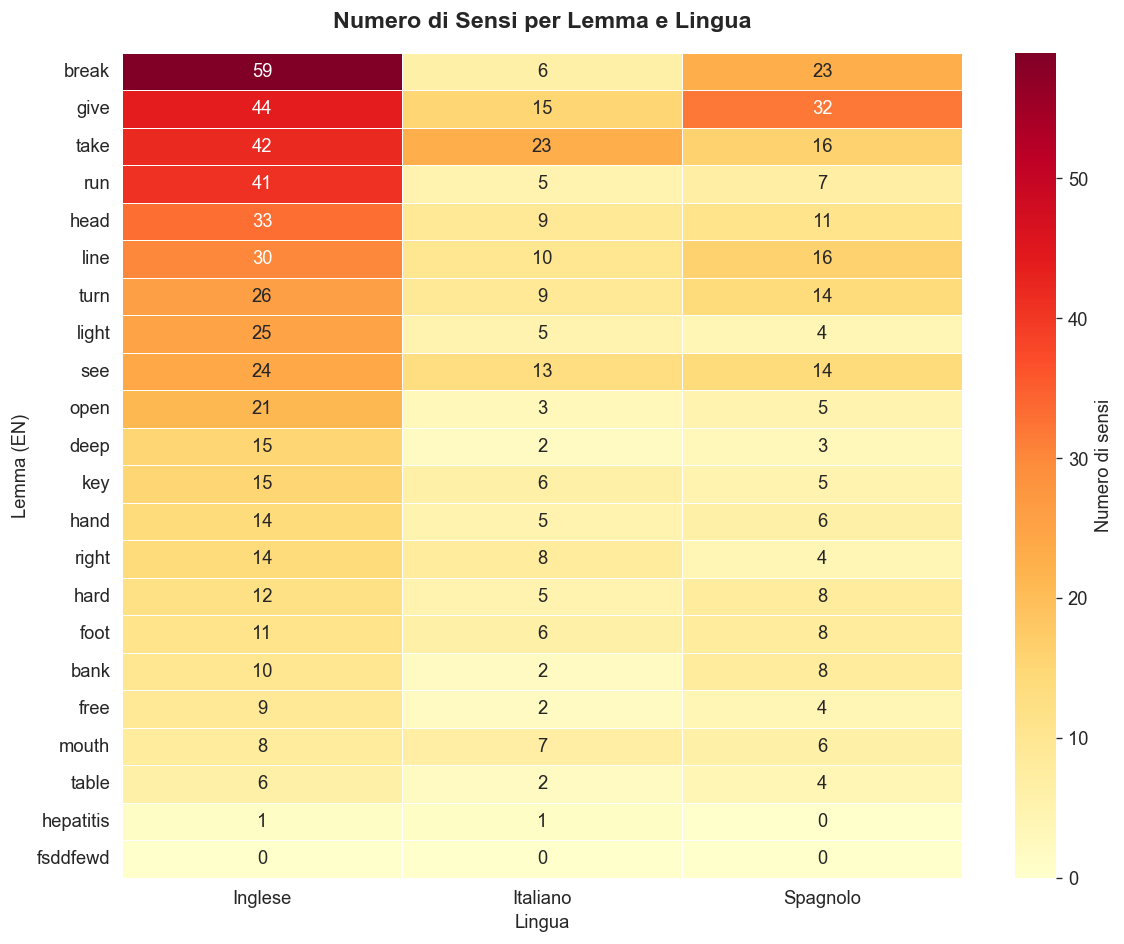
\includegraphics[width=0.85\textwidth]{heatmap_sensi.png}
  \caption{Numero di sensi per ciascuno dei 20 lemmi, nelle tre lingue. I lemmi sono ordinati per numero di sensi in inglese (decrescente).}
  \label{fig:heatmap}
\end{figure}

La Figura~\ref{fig:heatmap} rende immediatamente visibile il pattern: la colonna ``Inglese'' \`e sistematicamente la pi\`u scura (valori pi\`u alti) per quasi tutti i lemmi, con \textit{break} (59 sensi) e \textit{run} (41) come casi estremi. Le colonne italiana e spagnola sono molto pi\`u chiare, ma con alcune eccezioni interessanti discusse in Sez.~\ref{sec:discussione}.

\subsection{Entropia polisemica per lemma e lingua}

\begin{figure}[H]
  \centering
  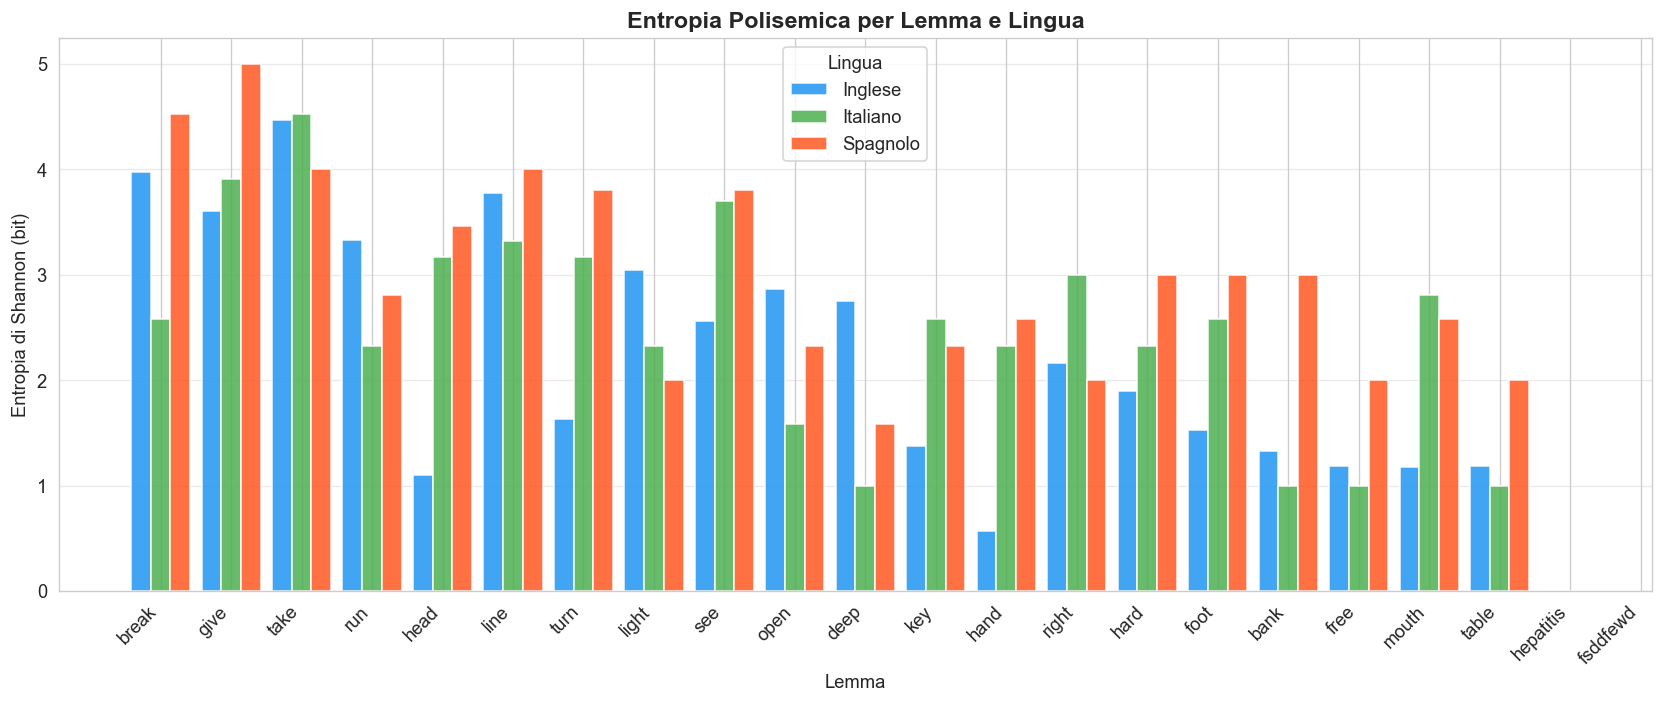
\includegraphics[width=0.95\textwidth]{barplot_entropia.png}
  \caption{Entropia di Shannon (bit) per ciascun lemma, confrontata tra le tre lingue (SemCor per l'inglese, uniforme per IT/ES).}
  \label{fig:entropia}
\end{figure}

Per italiano e spagnolo, essendo l'entropia calcolata come $\log_2 n$ sotto l'ipotesi di uniformit\`a, il loro andamento nella Figura~\ref{fig:entropia} ricalca esattamente quello dell'heatmap ma in scala logaritmica -- utile per confrontare la \emph{complessit\`a percepita} piuttosto che il conteggio grezzo, ma senza aggiungere informazione indipendente da $n$. Per l'inglese, invece, le barre \emph{non} sono una trasformazione monotona del numero di sensi: un lemma con molti sensi pu\`o avere entropia reale bassa se l'uso \`e concentrato (es.\ \textit{head}, Sez.~\ref{sec:entropia-vs-log2n}), rendendo il barplot inglese l'unico dei tre a portare informazione genuinamente distinta da quella della Figura~\ref{fig:heatmap}.

\subsection{Asimmetria EN vs.\ lingue romanze}

\begin{figure}[H]
  \centering
  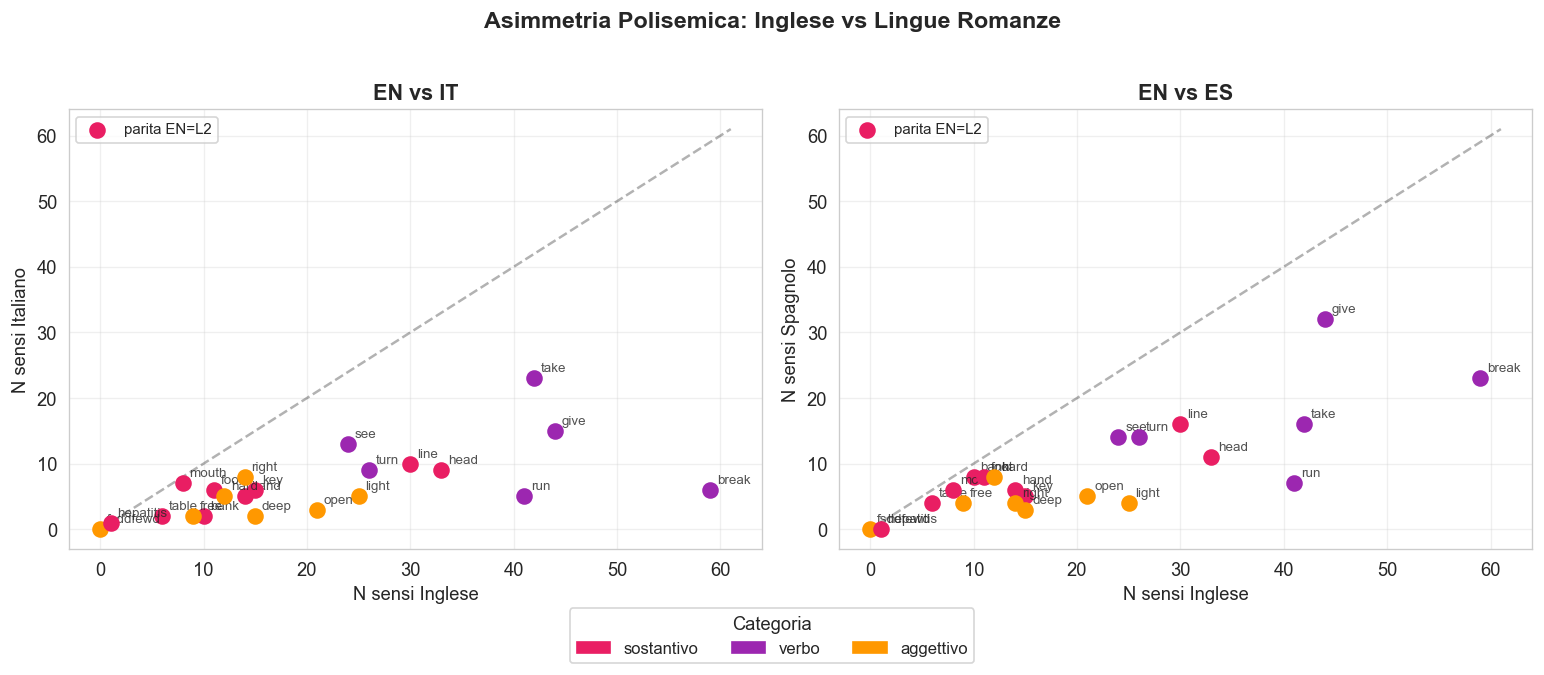
\includegraphics[width=\textwidth]{scatter_asimmetria.png}
  \caption{Numero di sensi in inglese contro italiano (sinistra) e spagnolo (destra). La linea diagonale tratteggiata indica parit\`a; i punti colorati per categoria grammaticale.}
  \label{fig:scatter}
\end{figure}

Tutti i punti in Figura~\ref{fig:scatter} si trovano \textbf{sistematicamente sotto la diagonale di parit\`a}, in entrambi i pannelli: per nessuno dei 20 lemmi l'italiano o lo spagnolo risultano pi\`u polisemici dell'inglese. La dispersione \`e maggiore nel pannello EN-ES che in quello EN-IT, coerentemente con la media pi\`u alta dello spagnolo (9.90 vs 7.15) osservata in Sez.~4.1.

\begin{table}[H]
  \centering
  \caption{Top 5 lemmi per asimmetria cross-linguistica (max$-$min sensi, dati reali)}
  \begin{tabular}{lrrrrr}
    \toprule
    \textbf{Lemma (EN)} & \textbf{Inglese} & \textbf{Italiano} & \textbf{Spagnolo} & \textbf{Asimmetria} & \textbf{EN/IT} \\
    \midrule
    break & 59 & 6  & 23 & 53 & 9.83$\times$ \\
    run   & 41 & 5  & 7  & 36 & 8.20$\times$ \\
    give  & 44 & 15 & 32 & 29 & 2.93$\times$ \\
    take  & 42 & 23 & 16 & 26 & 1.83$\times$ \\
    head  & 33 & 9  & 11 & 24 & 3.67$\times$ \\
    \bottomrule
  \end{tabular}
\end{table}

\begin{table}[H]
  \centering
  \caption{Lemmi con minore asimmetria (comportamento pi\`u simile tra lingue, dati reali)}
  \begin{tabular}{lrrrr}
    \toprule
    \textbf{Lemma (EN)} & \textbf{Inglese} & \textbf{Italiano} & \textbf{Spagnolo} & \textbf{Asimmetria} \\
    \midrule
    mouth & 8  & 7 & 6 & 2 \\
    table & 6  & 2 & 4 & 4 \\
    foot  & 11 & 6 & 8 & 5 \\
    hard  & 12 & 5 & 8 & 7 \\
    free  & 9  & 2 & 4 & 7 \\
    \bottomrule
  \end{tabular}
\end{table}

\subsection{Distribuzione per lingua e categoria grammaticale}

\begin{figure}[H]
  \centering
  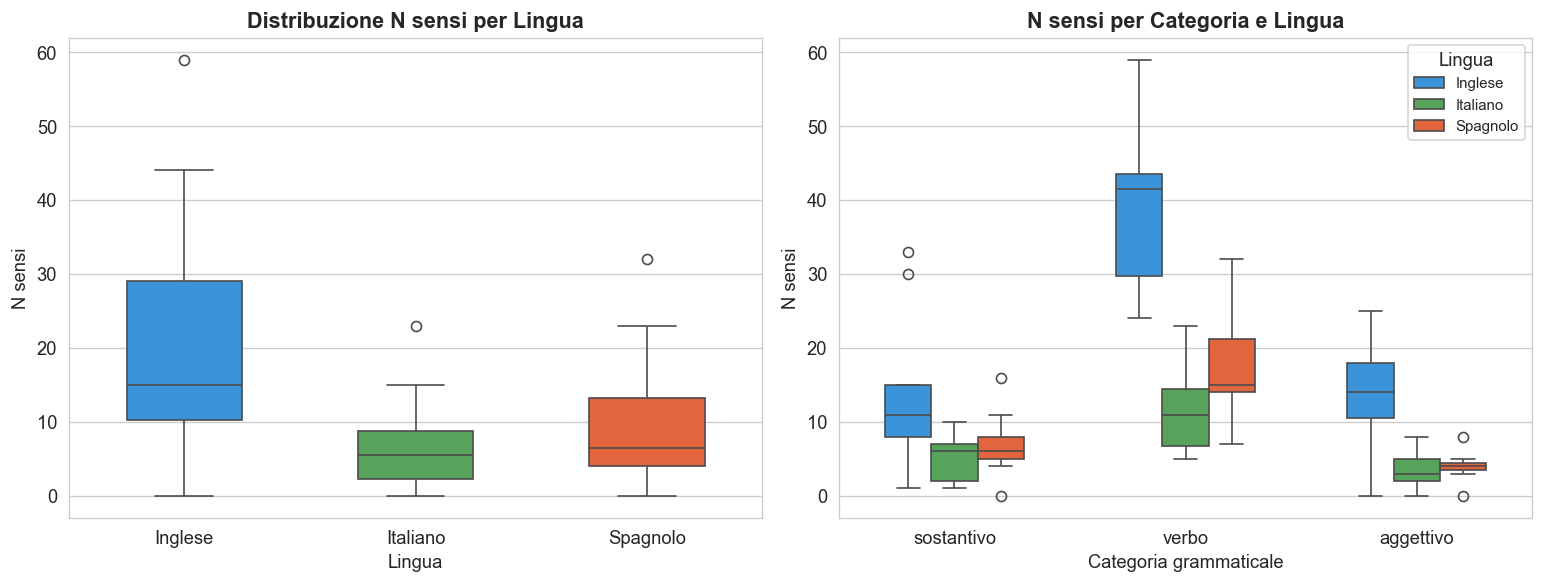
\includegraphics[width=\textwidth]{boxplot_distribuzione.png}
  \caption{Sinistra: distribuzione del numero di sensi per lingua. Destra: distribuzione per categoria grammaticale, confrontata tra lingue.}
  \label{fig:boxplot}
\end{figure}

Il pannello sinistro di Figura~\ref{fig:boxplot} confirma visivamente la gerarchia EN $\gg$ ES $>$ IT con box ben separati e poca sovrapposizione. Il pannello destro mostra che la gerarchia si mantiene \textbf{all'interno di ogni categoria grammaticale} (sostantivi, verbi, aggettivi), suggerendo che il fenomeno non \`e un artefatto della scelta di una particolare classe di parole, ma una caratteristica strutturale della differenza tra le risorse lessicali delle tre lingue in OMW.

\subsection{Rapporti di polisemia}

\begin{figure}[H]
  \centering
  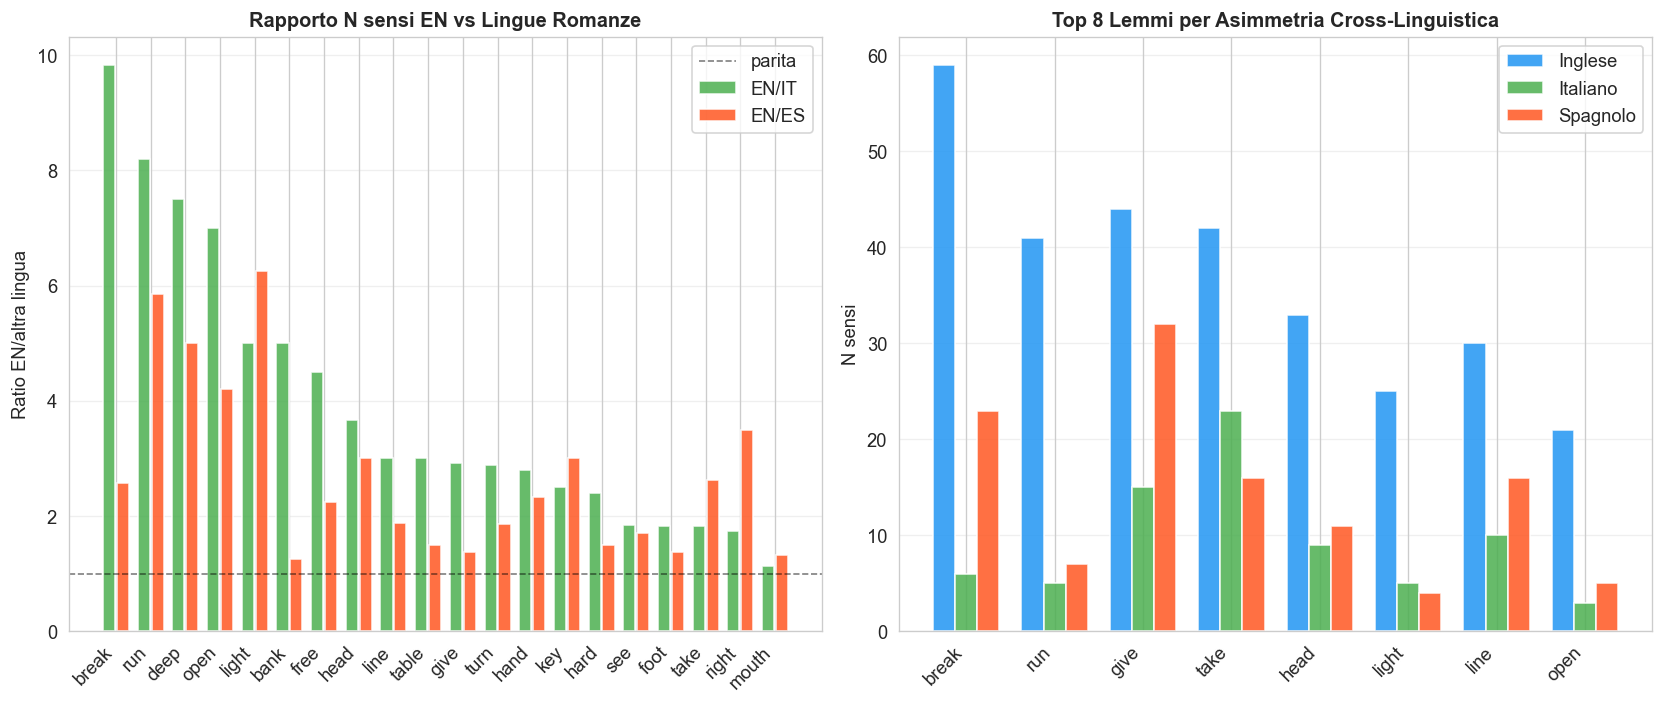
\includegraphics[width=\textwidth]{asimmetrie.png}
  \caption{Sinistra: rapporto EN/IT ed EN/ES per ciascun lemma. Destra: confronto diretto del numero di sensi per i 8 lemmi pi\`u asimmetrici.}
  \label{fig:asimmetrie}
\end{figure}

Il pannello sinistro di Figura~\ref{fig:asimmetrie} mostra che per il lemma \textit{break} il rapporto EN/IT raggiunge $9.83$ (59 sensi inglesi contro 6 italiani), il pi\`u alto fra i 20 lemmi; per \textit{run} il rapporto EN/ES \`e $5.86$ (41 contro 7). Questi valori estremi confermano quantitativamente l'intuizione qualitativa delle dispense: ``la stessa area semantica pu\`o essere lessicalizzata in modi diversi'' -- in questo caso, l'inglese concentra un numero molto maggiore di accezioni sotto un'unica forma lessicale.

% ============================================================
\section{Discussione}
\label{sec:discussione}
% ============================================================

\subsection{L'entropia reale rivela ambiguit\`a d'uso che il conteggio dei sensi nasconde}
\label{sec:entropia-vs-log2n}

La disponibilit\`a di un'entropia \emph{reale} (da SemCor) solo per l'inglese permette un confronto diretto, sui 20 lemmi inglesi, fra l'entropia osservata e quella che si otterrebbe assumendo (come per IT/ES) una distribuzione uniforme, $\log_2 n$. La correlazione fra le due misure \`e $r=0.76$: alta, ma tutt'altro che 1 -- il numero di sensi e l'ambiguit\`a d'uso reale sono quantit\`a correlate ma distinte. Gli scarti pi\`u ampi sono istruttivi:

\begin{table}[H]
  \centering
  \caption{Lemmi inglesi con maggiore scarto fra entropia reale ed entropia uniforme $\log_2 n$}
  \begin{tabular}{lrrrrr}
    \toprule
    \textbf{Lemma} & \textbf{$n$ sensi} & \textbf{Entropia reale} & \textbf{$\log_2 n$} & \textbf{Scarto} & \textbf{Quota senso dominante} \\
    \midrule
    head & 33 & 1.10 bit & 5.04 bit & 3.94 bit & 82\% \\
    hand & 14 & 0.56 bit & 3.81 bit & 3.24 bit & 93\% \\
    turn & 26 & 1.63 bit & 4.70 bit & 3.07 bit & 74\% \\
    key  & 15 & 1.38 bit & 3.91 bit & 2.53 bit & 67\% \\
    \bottomrule
  \end{tabular}
\end{table}

\textit{Head} ha 33 sensi catalogati in WordNet, ma l'82\% delle occorrenze reali in SemCor usa un unico senso dominante (verosimilmente ``parte del corpo''): l'entropia reale (1.10 bit) \`e quasi cinque volte pi\`u bassa di quella che il solo conteggio dei sensi (5.04 bit) suggerirebbe. \textit{Hand} \`e ancora pi\`u estremo: 14 sensi ma il 93\% dell'uso concentrato su un solo senso. All'estremo opposto, lemmi come \textit{take} (42 sensi, entropia reale 4.47 bit, quota del senso dominante appena 12.6\%) o \textit{break} (59 sensi, 3.98 bit, 15.8\%) mostrano un'ambiguit\`a d'uso che \emph{corrisponde} effettivamente all'alto numero di sensi catalogati. In altre parole: un numero di sensi elevato \`e condizione necessaria ma non sufficiente per un'ambiguit\`a d'uso elevata, e solo l'entropia calcolata su dati di frequenza reali pu\`o distinguere i due casi -- esattamente il limite gi\`a segnalato in Sez.~\ref{sec:entropia-metodo} a proposito di IT/ES, per cui questa distinzione resta strutturalmente invisibile.

\subsection{La gerarchia EN $\gg$ ES $>$ IT non \`e (solo) linguistica}

Il risultato pi\`u robusto -- la media di 22.95 sensi in inglese contro 9.90 in spagnolo e 7.15 in italiano -- deve essere interpretato con cautela. Princeton WordNet (la base della parte inglese di OMW) \`e una risorsa costruita e raffinata per oltre 30 anni da linguisti computazionali, con una granularit\`a dei sensi spesso molto fine (lo stesso problema della granularit\`a discusso nelle dispense, Cap.~1: WordNet distingue sensi che un parlante non percepirebbe come distinti). Le estensioni multilingue di OMW per italiano e spagnolo sono invece mappature pi\`u recenti e meno esaustive. Una parte della differenza osservata \`e quindi plausibilmente dovuta a \textbf{differenze nella copertura e nella granularit\`a delle risorse}, non solo a una reale differenza di polisemia tra le lingue -- una limitazione importante da segnalare, in linea con l'invito delle dispense a non considerare il numero di sensi nel dizionario come misura definitiva (Cap.~4: ``una parola pu\`o avere molti sensi nel dizionario, ma usarne abitualmente solo pochi''), un invito che l'analisi di Sez.~\ref{sec:entropia-vs-log2n} rende ora operativo (almeno per l'inglese) invece che puramente qualitativo.

\subsection{Il caso \textit{bank}: asimmetria semantica, non solo quantitativa}

Il lemma \textit{bank} (10 sensi nominali EN, entropia reale 1.32 bit, quota del senso dominante 52\%; 2 IT, entropia 1.00 bit; 8 ES, entropia uniforme 3.00 bit) \`e istruttivo non solo per il numero ma per la \textbf{struttura} dei sensi. L'entropia reale conferma che, anche in inglese, l'uso di \textit{bank} \`e dominato da un solo senso (verosimilmente l'istituto finanziario) nonostante 10 sensi catalogati. In italiano, ``banca'' (2 sensi) copre quasi esclusivamente lo stesso istituto finanziario: il senso ``riva del fiume'' \`e lessicalizzato in una parola completamente diversa (\textit{riva}), non tracciata in questo studio per il lemma \textit{bank}. In spagnolo, invece, ``banco'' (8 sensi) \`e semanticamente pi\`u carico: copre l'istituto finanziario, ma anche il mobile (panca/banco di scuola) e il banco di sabbia/pesci -- un comportamento pi\`u vicino a quello inglese, dove \textit{bank} include gi\`a il significato geografico oltre a quello finanziario. Questo \`e un esempio concreto di \textbf{asimmetria cross-linguistica nella lessicalizzazione}: la stessa area concettuale viene divisa diversamente tra le tre lingue, esattamente il fenomeno teorizzato nelle dispense con l'esempio italiano ``tempo'' (atmosferico + cronologico) vs.\ l'inglese (\textit{weather}/\textit{time} separati).

\subsection{Verbi vs sostantivi concreti: la categoria grammaticale spiega parte dell'asimmetria}

Aggregando per categoria grammaticale (Tabella~\ref{tab:categoria}) emerge un pattern netto: i verbi inglesi hanno in media \textbf{39.33 sensi}, contro 15.88 dei sostantivi e 16.00 degli aggettivi -- pi\`u del doppio. La stessa gerarchia (verbi $>$ aggettivi $\approx$ sostantivi) si mantiene in italiano (11.83 vs 5.88 vs 4.17) e spagnolo (17.67 vs 8.00 vs 4.67), ma con un divario assoluto molto pi\`u ampio in inglese: la differenza fra verbi e sostantivi \`e di 23.45 sensi in inglese, contro 5.95 in italiano e 9.67 in spagnolo.

\begin{table}[H]
  \centering
  \caption{Numero medio di sensi per categoria grammaticale e lingua}
  \label{tab:categoria}
  \begin{tabular}{lrrr}
    \toprule
    \textbf{Categoria} & \textbf{Inglese} & \textbf{Italiano} & \textbf{Spagnolo} \\
    \midrule
    Verbo      & 39.33 & 11.83 & 17.67 \\
    Aggettivo  & 16.00 &  4.17 &  4.67 \\
    Sostantivo & 15.88 &  5.88 &  8.00 \\
    \bottomrule
  \end{tabular}
\end{table}

I due lemmi con asimmetria pi\`u estrema sono infatti entrambi verbi: \textit{break} (53) e \textit{run} (36). Questo \`e in linea con l'osservazione delle dispense secondo cui i verbi tendono a presentare ``polisemia molto elevata'' in inglese (lo stesso esempio di \textit{run} \`e citato esplicitamente nel Cap.~4 delle dispense). Il verbo inglese \textit{run} si estende infatti a domini semantici molto eterogenei -- corsa fisica, gestione (\textit{run a business}), funzionamento di macchine (\textit{the engine runs}), candidatura politica (\textit{run for office}), liquidi che scorrono -- ciascuno dei quali in italiano e spagnolo \`e tipicamente lessicalizzato con un verbo distinto (\textit{correre}, \textit{gestire}, \textit{funzionare}, \textit{candidarsi}, \textit{scorrere}), motivando direttamente il basso numero di sensi rilevato per ``correre''/``correr'' (5 e 7 rispettivamente), che in OMW intercetta solo l'accezione di movimento fisico. Sui 5 lemmi a maggiore asimmetria (Tabella~3), 4 su 5 sono verbi (\textit{break}, \textit{run}, \textit{give}, \textit{take}; l'unica eccezione \`e il sostantivo \textit{head}), confermando quantitativamente che la categoria grammaticale non \`e un dettaglio metodologico ma un fattore esplicativo di primo ordine dell'asimmetria osservata.

\subsection{I lemmi pi\`u stabili cross-linguisticamente}

All'estremo opposto, \textit{mouth} (asimmetria 2) e \textit{table} (asimmetria 4) mostrano il comportamento pi\`u omogeneo tra le lingue. Si tratta di due sostantivi concreti con un referente fisico ben definito (la bocca, il tavolo): coerentemente con quanto discusso a proposito dei concetti \textbf{Concrete Generic/Specific} nei laboratori 1-2, il vincolo del referente fisico limita anche la variabilit\`a del numero di estensioni di significato disponibili, in tutte e tre le lingue. Da notare che tutti e 5 i lemmi a minore asimmetria (Tabella~4) sono sostantivi o aggettivi -- mai verbi -- un'ulteriore conferma, in negativo, del pattern discusso in Sez.~4.5.

\subsection{Implicazioni per il NLP multilingue}

I risultati confermano in modo quantitativo le implicazioni discusse nelle dispense (Cap.~4.5.3): un sistema di \textbf{machine translation} o di \textbf{cross-lingual transfer} che assuma una corrispondenza 1:1 tra i sensi di un lemma inglese e quelli del corrispettivo italiano o spagnolo commetterebbe un errore sistematico, specialmente per verbi ad alta polisemia come \textit{run} o \textit{break}: un modello addestrato sulla granularit\`a fine di WordNet inglese, se applicato senza adattamento a un dominio italiano o spagnolo, tender\`a a generare ambiguit\`a spurie o a fallire nel mappare correttamente le accezioni. L'analisi di Sez.~\ref{sec:entropia-vs-log2n} aggiunge una sfumatura pratica: per lemmi come \textit{head} o \textit{hand}, il rischio reale non \`e la genuina ambiguit\`a (che l'entropia mostra essere bassa), ma l'illusione di ambiguit\`a indotta dal solo conteggio dei sensi WordNet -- un sistema che trattasse ogni senso catalogato come ugualmente probabile sovrastimerebbe sistematicamente la difficolt\`a di disambiguazione per questi lemmi.

% ============================================================
\section{Conclusioni}
% ============================================================

Il laboratorio ha verificato empiricamente, su 20 lemmi e tre lingue, la tesi delle dispense secondo cui \textbf{non esiste una polisemia universale}: il numero di sensi disponibili per lo stesso lemma varia sistematicamente tra inglese, italiano e spagnolo (rispettivamente 22.95, 7.15 e 9.90 sensi medi, con filtro di categoria grammaticale applicato in ogni query), con asimmetrie individuali fino a $9.83\times$ (\textit{break}, EN/IT) e $5.86\times$ (\textit{run}, EN/ES).

I risultati principali sono:

\begin{enumerate}
  \item \textbf{Gerarchia sistematica EN $\gg$ ES $>$ IT}, confermata sia nell'aggregato sia all'interno di ogni categoria grammaticale (sostantivi, verbi, aggettivi) -- ma da interpretare cum grano salis, essendo in parte attribuibile a differenze di copertura/granularit\`a tra le risorse lessicali, non solo a una reale differenza di polisemia.
  \item \textbf{L'entropia reale (SemCor) rivela ambiguit\`a d'uso non deducibile dal conteggio dei sensi}: la correlazione fra entropia reale e $\log_2 n$ sui 20 lemmi inglesi \`e $r=0.76$, non 1. Lemmi come \textit{head} (33 sensi, ma 82\% di uso concentrato su un solo senso) sono formalmente polisemici ma praticamente quasi monosemici in uso; lemmi come \textit{take} o \textit{break} sono invece genuinamente ambigui, con l'uso distribuito su molti sensi.
  \item \textbf{I verbi mostrano l'asimmetria pi\`u marcata} (media 39.33 sensi EN contro 11.83 IT e 17.67 ES), coerentemente con la tendenza dei verbi inglesi a un'estensione semantica molto ampia rispetto alle lingue romanze; 4 dei 5 lemmi pi\`u asimmetrici sono verbi.
  \item \textbf{I sostantivi concreti con referente fisico stabile} (\textit{mouth}, \textit{table}, \textit{foot}) mostrano la minore asimmetria cross-linguistica, suggerendo che il vincolo referenziale limiti la variabilit\`a anche a livello multilingue.
  \item \textbf{L'asimmetria non \`e solo quantitativa ma strutturale}: il caso \textit{bank}/\textit{banca}/\textit{banco} mostra come la stessa area concettuale possa essere ripartita in modo diverso tra parole distinte (italiano) o concentrata in un'unica forma pi\`u carica semanticamente (spagnolo, pi\`u vicino all'inglese) -- e l'entropia reale conferma che, comunque la si ripartisca, l'uso resta dominato da un unico senso in tutte e tre le lingue.
\end{enumerate}

Il limite principale dello studio resta l'assunzione di \textbf{distribuzione uniforme dei sensi} per italiano e spagnolo, dovuta all'assenza di dati di frequenza d'uso in OMW per queste due lingue (a differenza dell'inglese, dove tali dati esistono via SemCor e sono stati effettivamente usati in questa versione dello studio). Un'estensione naturale del lavoro sarebbe integrare stime di frequenza anche per le lingue romanze (es.\ da corpora annotati o da conteggi su corpora di testo generici), permettendo di verificare se il pattern osservato per l'inglese in Sez.~\ref{sec:entropia-vs-log2n} -- sensi numerosi ma uso concentrato per alcuni lemmi -- si replichi anche in italiano e spagnolo, e di distinguere lemmi con \emph{molti sensi ma fortemente dominati da un uso comune} da lemmi con sensi realmente equiprobabili in tutte e tre le lingue, non solo in inglese.

\end{document}
